\documentclass[a4paperm]{article}
%\documentclass[12pt,twocolumn]{article}

\usepackage[T2A]{fontenc}
\usepackage[utf8]{inputenc}
\usepackage[russian,english]{babel}
\usepackage{amsmath,amsthm,amssymb,stackrel}
\usepackage[affil-it]{authblk}
\usepackage{cite}
\usepackage{scrextend}
\usepackage{verbatim}
\usepackage{paralist}
\usepackage[mediumspace,mediumqspace,Grey,squaren]{SIunits}
\addtokomafont{labelinglabel}{\sffamily}
\usepackage{amsmath}
\usepackage{graphicx}
 \usepackage[usenames, dvipsnames]{color}
 \usepackage{multirow}
 \usepackage{longtable}
 \usepackage{lineno}
 \usepackage{textcomp}
 
 \usepackage{xr}
 
 
%\usepackage[none]{hyphenat} %no nyphenation

\usepackage{SIunits}
\usepackage{miller}
\usepackage[version=3]{mhchem}

\usepackage{float} %H with figures

\setlength{\parindent}{5ex}

 \usepackage{newfloat} %For numbering of supplemmentary figures

\graphicspath{{../figures/}}

\usepackage[outdir=figures/]{epstopdf}


\externaldocument[supp]{supplementary/supp}

\renewcommand{\thefigure}{S\arabic{figure}}
\renewcommand{\thetable}{S\arabic{table}}



\begin{document}

%\linenumbers


\title{Supporting Information}
\title{Janus structures of SMoSe and SVSe compositions with low enthalpy and unusual crystal chemistry}


\author[1,2,3]{Pavel N. Gavryushkin
   \thanks{Electronic address: \texttt{gavryushkin@igm.nsc.ru, p.gavryushkin@g.nsu.ru}; Corresponding author}}     
\author[2]{Nursultan Sagatov}
\author[1]{Ekaterina V. Sukhanova}
\author[4]{Inna V. Medrish}
\author[1]{Zakhar I. Popov}

\affil[1]{Emanuel Institute of Biochemical Physics of Russian Academy of Sciences, 4 Kosygin Street, Moscow, 119334, Russian Federation}
\affil[2]{Sobolev Institute of Geology and Mineralogy, Siberian Branch of Russian Academy of Sciences, prosp. acad. Koptyuga 3, 630090 Novosibirsk, Russian Federation}
\affil[3]{Novosibirsk State University, Pirogova 2, Novosibirsk 630090, Russian Federation}
\affil[4]{Samara Center for Theoretical Material Science (SCTMS), Samara State Technical University, Molodogvardeyskaya St. 244, Samara, Russia 443100}


\date{}
\maketitle

%\linenumbers


\begin{table}[H]
	\caption{Structural data SMoSe-O, O', and M''.} \label{t:str_test} \vspace{2mm}
	\centering
	\begin{tabular}{l*{9}{l}}
		\hline
		\multirow{2}*{Phase}	& 	\multirow{2}*{Space group}	& \multicolumn{3}{c}{\multirow{2}*{Lattice parameters (\AA, deg)}}	&	\multirow{2}*{Atom}	&	\multicolumn{3}{c}{Coordinates} \\ 
		\cline{7-9}
		&&&&&&  x	&	y	&	z \\ 
		\hline 
		SMoSe & $Pmm2\ (\#25)$  &	$a=5.6497$ & $b=3.2416$ & $c=23.0295$  & Mo	&	0.2432	&	0.5	&	0.5028	\\
		test-1&&$\alpha$ = 90.000& $\beta$=90.000& $\gamma$=90.000& S	&	0.0000	&	0	&	0.5628	\\
		&&&&&	S	&	0.5000	&	0.5	&	0.5815	\\
		&&&&&	Se	&	0.0000	&	0	&	0.4342	\\
		&&&&&	Se	&	0.5000	&	0.5	&	0.4159	\\
		\hline
		SMoSe & $Pmm2\ (\#25)$  &	$a=11.8737$ & $b=3.1617$ & $c=26.1470$  & Mo	&	0.1113	&	0.5	&	0.5006	\\
		test-2&&$\alpha$ = 90.000& $\beta$=90.000& $\gamma$=90.000& Mo	&	0.3330	&	0	&	0.5000	\\
		&&&&&	S	&	0.0000	&	0	&	0.5563	\\
		&&&&&	S	&	0.5000	&	0	&	0.5516	\\
		&&&&&	S	&	0.2605	&	0.5	&	0.5618	\\
		&&&&&	Se	&	0.0000	&	0	&	0.4385	\\
		&&&&&	Se	&	0.5000	&	0	&	0.4377	\\
		&&&&&	Se	&	0.2573	&	0.5	&	0.4319	\\
		\hline
		SMoSe & $Pm\ (\#6)$  &	$a=6.4527$ & $b=9.3860$ & $c=25.1952$  & Mo	&	0.0177	&	0.7861	&	0.4954	\\
		test-3&&$\alpha$ = 90.000& $\beta$=90.179& $\gamma$=90.000& Mo	&	0.4825	&	0.7898	&	0.4967	\\		
		&&&&&	Mo	&	0.3301	&	0.5000	&	0.4961	\\
		&&&&&	Mo	&	0.6747	&	0.5000	&	0.4970	\\
		&&&&&	S	&	0.0102	&	0.0000	&	0.4509	\\
		&&&&&	S	&	0.4903	&	0.0000	&	0.4433	\\
		&&&&&	S	&	0.7476	&	0.6923	&	0.4359	\\
		&&&&&	S	&	0.2535	&	0.6859	&	0.4320	\\
		&&&&&	Se	&	0.0605	&	0.0000	&	0.5646	\\
		&&&&&	Se	&	0.4419	&	0.0000	&	0.5639	\\
		&&&&&	Se	&	0.7490	&	0.7008	&	0.5648	\\
		&&&&&	Se	&	0.2508	&	0.6822	&	0.5673	\\
		\hline
	\end{tabular}
\end{table}


\begin{figure}[H]
	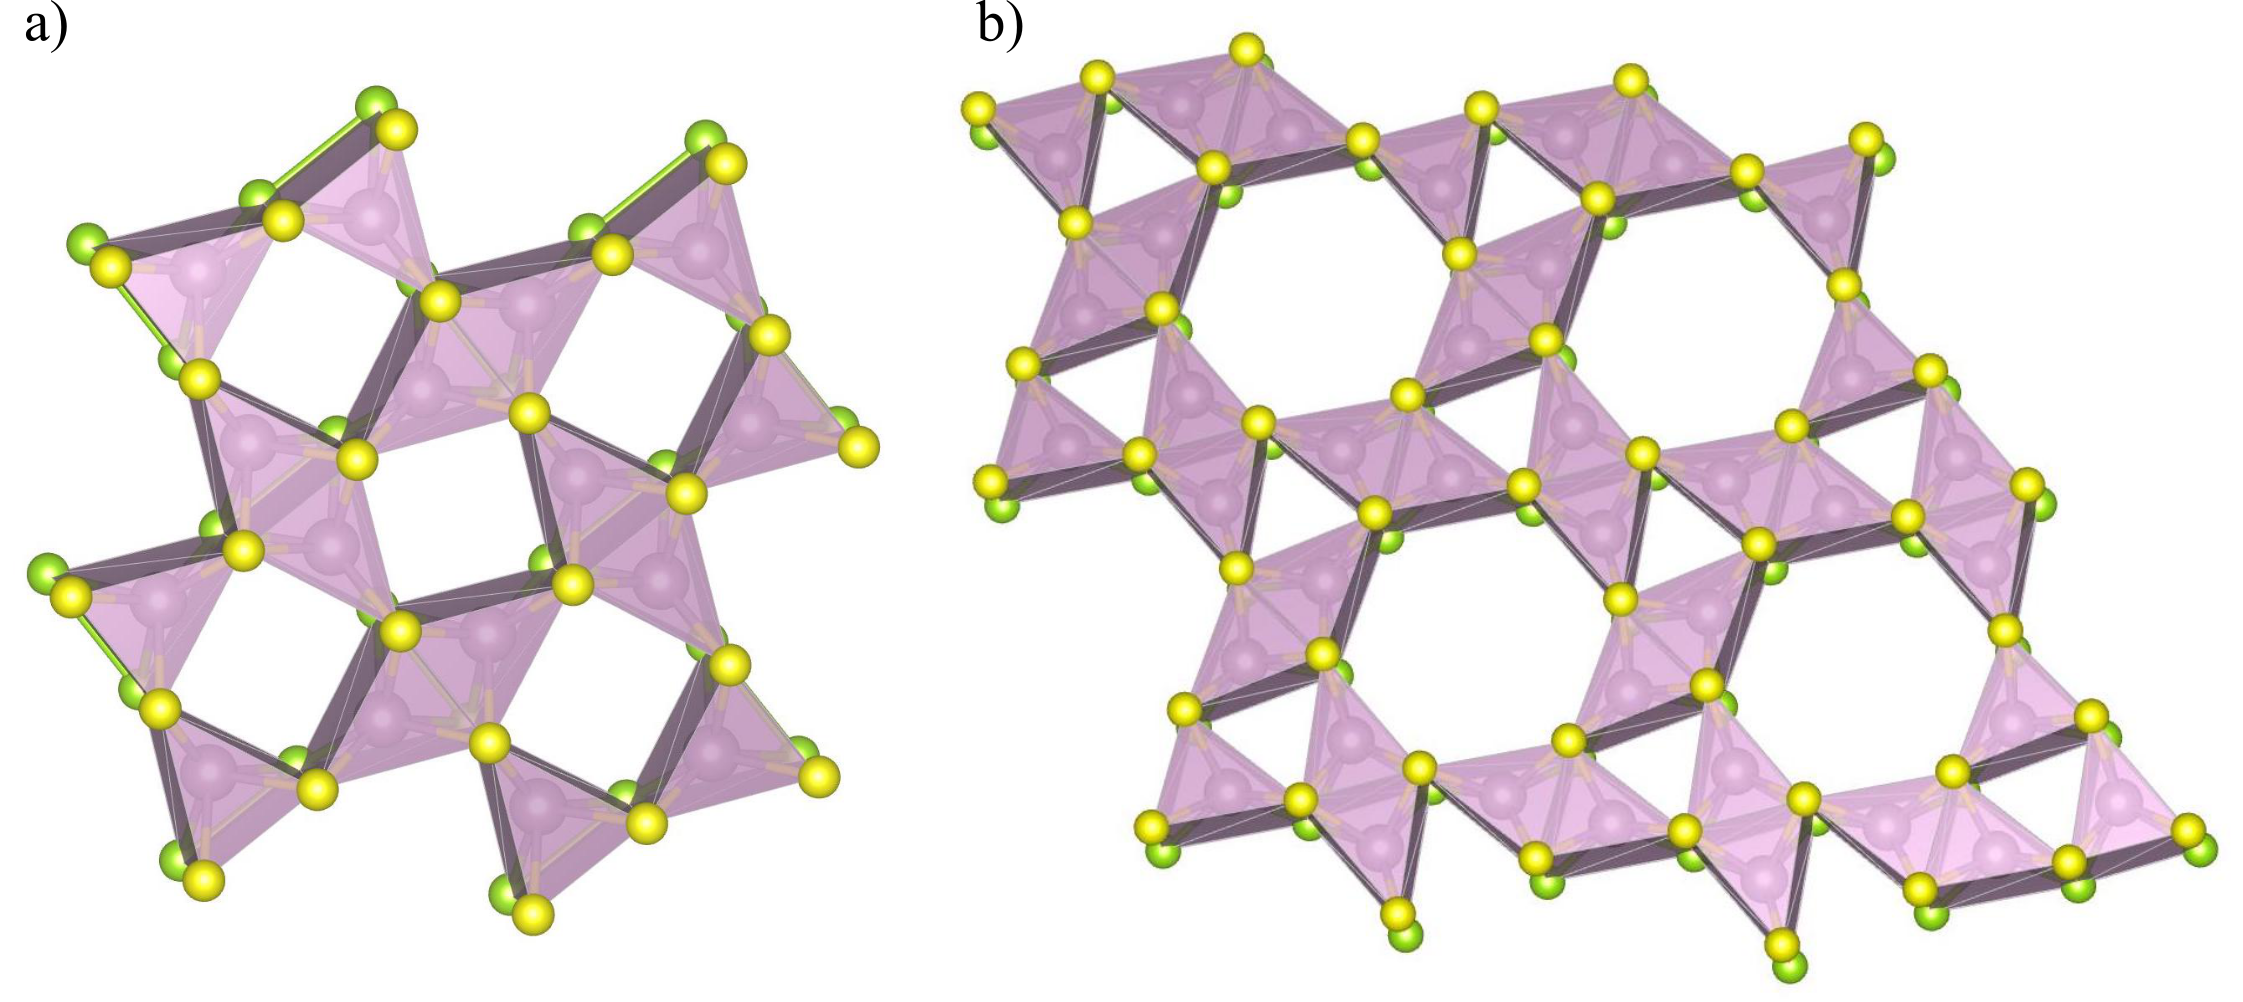
\includegraphics[width=\textwidth]{fes_fxt.png}
	\caption{Packing of trigonal prisms in 1S (a) and 1H' (b) structures of SMoSe.}
	\label{fes_fxt}
\end{figure}

\begin{figure}[H]
	\includegraphics[width=0.5\textwidth]{T_hor_ch.png} \\
	\caption{Comparison of the nets of Ch atoms in 1M (a) and 1T (b) crystal structures; sulphur is shown in yellow, selenium -- in green.}
	\label{T_hor_ch}
\end{figure}

\begin{figure}
	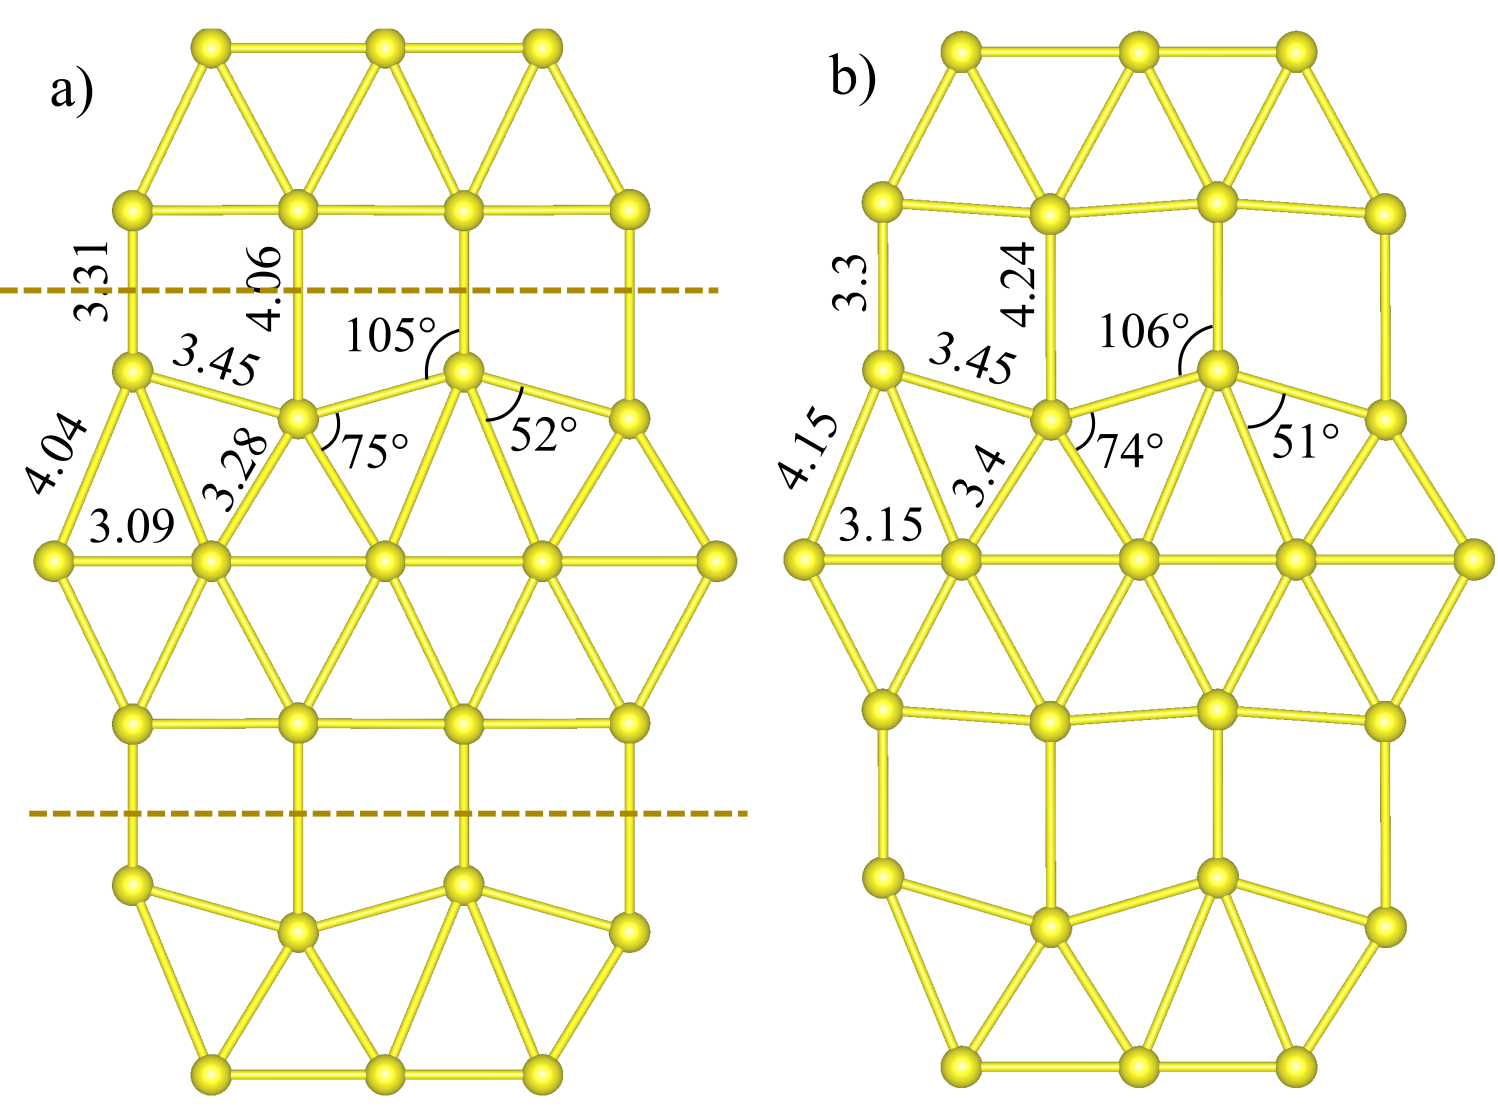
\includegraphics[width=0.85\textwidth]{airss1_s_comp.png}
	\caption{Interatomic distances and bond angles of sulphr nets in SVSe-1A (a) and SMoSe-1A' (b).}
	\label{airss1_s_comp}
\end{figure}

\begin{figure}[H]
	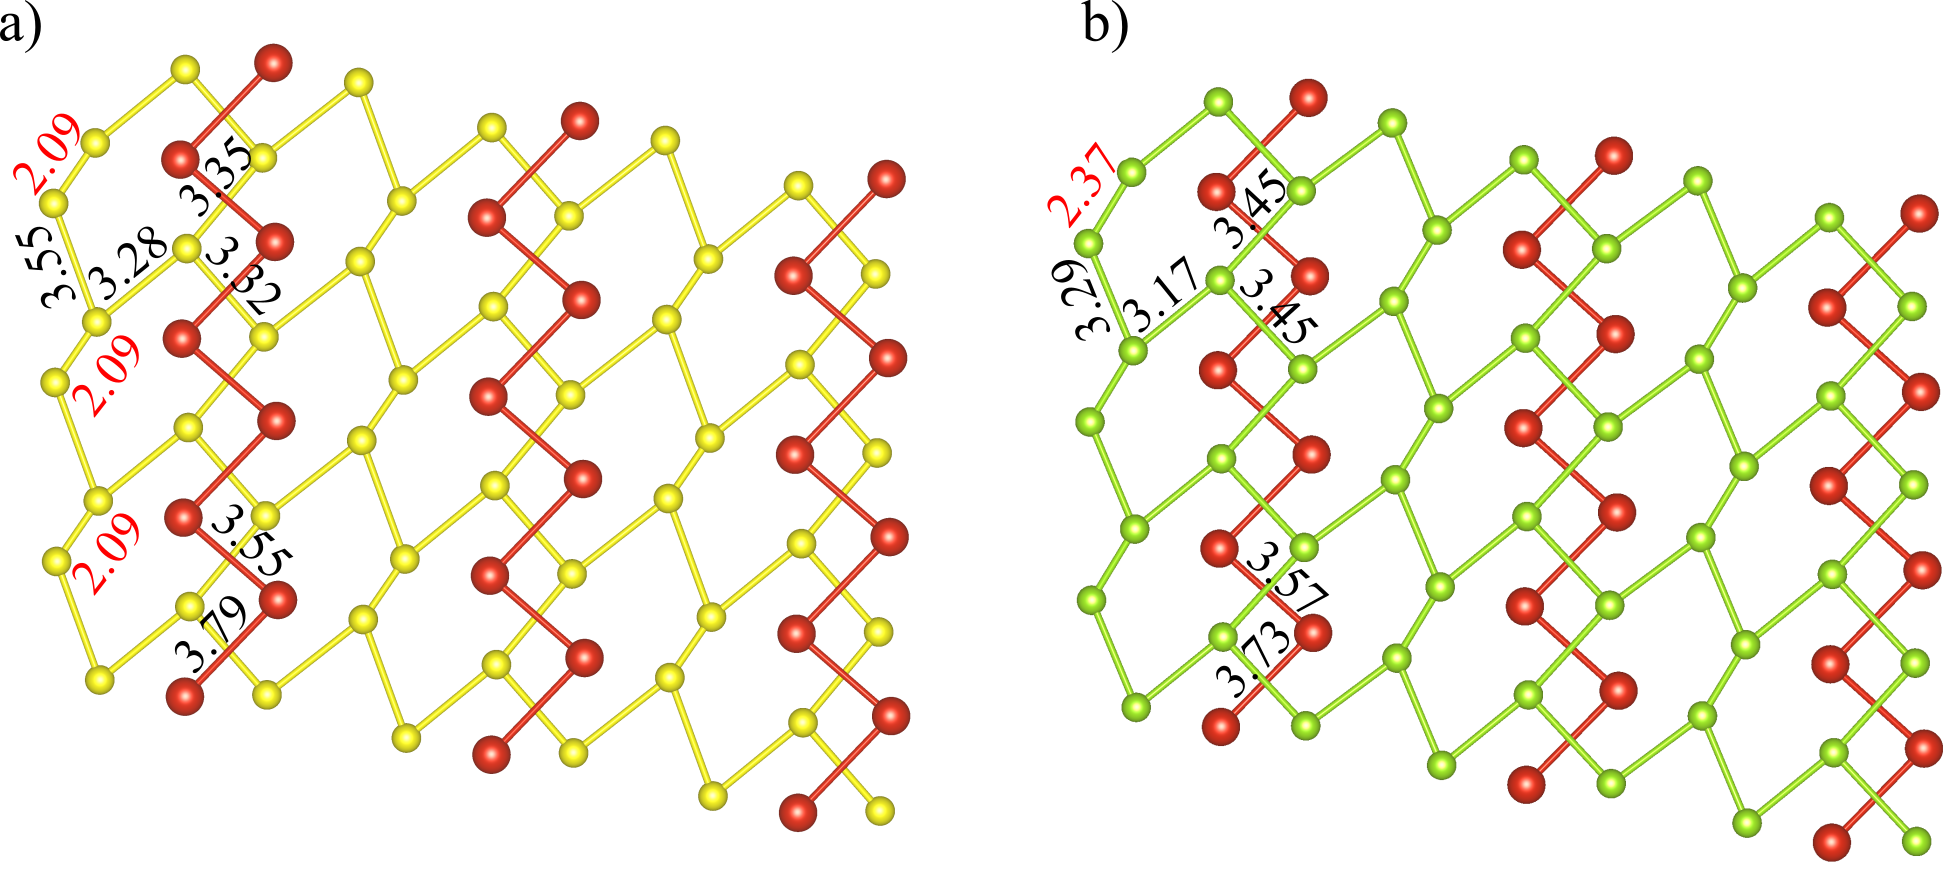
\includegraphics[width=\textwidth]{airss3_S_Se.png}
	\caption{The net of sulphur (a) and selenium (b) atoms in SVSe-1A'' crystal structure.}
	\label{airss3_S_Se}
\end{figure}


\end{document}
